\documentclass[Main.tex]{subfiles}
\begin{document}






\section{Limits of Agreement}
% introduces
A third element of the Bland-Altman methodology, an interval known
as `limits of agreement' is introduced in \citet*{BA86}
(sometimes referred to in literature as 95\% limits of agreement).
Limits of agreement are used to assess whether the two methods of
measurement can be used interchangeably. \citet{BA86} refer to
this as the `equivalence' of two measurement methods. The specific purpose of the limits of
agreement must be
established clearly. \citet*{BA95} comment that the limits of agreement `how
far apart measurements by the two methods were likely to be for
most individuals', a definition echoed in their 1999 paper:

\begin{quote}"We can then say that nearly all pairs
	of measurements by the two methods will be closer together than
	these extreme values, which we call 95\% limits of agreement.
	These values define the range within which most differences
	between measurements by the two methods will lie."
\end{quote}

The limits of agreement (LoA) are computed by the following
formula:
\[
LoA = \bar{d} \pm 1.96 s_{d}
\]
with $\bar{d}$ as the estimate of the inter method bias, $s_{d}$
as the standard deviation of the differences and 1.96 is the 95\%
quantile for the standard normal distribution. (Some accounts of
Bland-Altman plots use a multiple of 2 standard deviations instead
for simplicity.)

The limits of agreement methodology assumes a constant level of bias throughout the range of measurements. Importantly the authors recommend prior determination of what would and would constitute acceptable
agreement, and that sample sizes should be predetermined to give an accurate conclusion. However \citet{mantha} highlights inadequacies in the correct application of limits of agreement, resulting in contradictory estimates limits of agreement in various papers.

\begin{quote}
	``How far apart measurements can be without causing difficulties
	will be a question of judgment. Ideally, it should be defined in
	advance to help in the interpretation of the method comparison and
	to choose the sample size \citep{BA86}".
\end{quote}


For the Grubbs `F vs C' comparison, these limits
of agreement are calculated as -0.132 for the upper bound, and
-1.08 for the lower bound. Figure 1.9 shows the resultant
Bland-Altman plot, with the limits of agreement shown in dashed
lines.


%\begin{figure}[h!]
%\begin{center}
%  \includegraphics[width=125mm]{GrubbsBAplot-LOA.jpeg}
%  \caption{Bland-Altman plot with limits of agreement}\label{GrubbsBAplot-noLOA}
%\end{center}
%\end{figure}

%But as \citet*{BA86} point out this may not be the case. Variants of the limits of agreement that overcome this
% problem shall be introduced in due course.


\section{Limits of Agreement}
% introduces
A third element of the Bland-Altman approach, an interval known
as `limits of agreement' is introduced in \citet*{BA86}
(sometimes referred to in literature as 95\% limits of agreement).
Limits of agreement are used to assess whether the two methods of
measurement can be used interchangeably. \citet{BA86} refer to
this as the `equivalence' of two measurement methods. The specific question to which limits of
agreement are intended as the answer to must be
established clearly. \citet*{BA95} comment that the limits of agreement show `how
far apart measurements by the two methods were likely to be for
most individuals', a definition echoed in their 1999 paper:

\begin{quote}``We can then say that nearly all pairs
	of measurements by the two methods will be closer together than
	these extreme values, which we call 95\% limits of agreement.
	These values define the range within which most differences
	between measurements by the two methods will lie."
\end{quote}

The limits of agreement (LoA) are computed by the following
formula:
\[
LoA = \bar{d} \pm 1.96 s_{d}
\]
with $\bar{d}$ as the estimate of the inter method bias, $s_{d}$
as the standard deviation of the differences and 1.96 (sometimes rounded to 2) is the 95\%
quantile for the standard normal distribution. The limits of agreement methodology assumes a constant level of bias throughout the range of measurements. Importantly the authors recommend prior determination of what would constitute acceptable
agreement, and that sample sizes should be predetermined to give an accurate conclusion. However \citet{mantha} highlight inadequacies in the correct application of limits of agreement, resulting in contradictory estimates of limits of agreement in various papers.

%\begin{quote}
%``How far apart measurements can be without causing difficulties
%will be a question of judgment. Ideally, it should be defined in
%advance to help in the interpretation of the method comparison and
%to choose the sample size \citep{BA86}".
%\end{quote}


For the Grubbs `F vs C' comparison, these limits
of agreement are calculated as -0.132 for the upper bound, and
-1.08 for the lower bound. Figure 1.9 shows the resultant
Bland-Altman plot, with the limits of agreement shown in dashed
lines.


\begin{figure}[h!]
	\begin{center}
		\includegraphics[width=125mm]{images/GrubbsBAplot-LOA.jpeg}
		\caption{Bland-Altman plot with limits of agreement}\label{GrubbsBAplot-noLOA}
	\end{center}
\end{figure}

%But as \citet*{BA86} point out this may not be the case. Variants of the limits of agreement that overcome this
% problem shall be introduced in due course.

\subsection{Inferences on Bland-Altman estimates}
\citet*{BA99} advises on how to calculate confidence intervals for the inter-method bias and limits of agreement.
For the inter-method bias, the confidence interval is a simply that of a mean: $\bar{d} \pm t_{(\alpha/2,n-1)} S_{d}/\sqrt{n}$.
The confidence
intervals and standard error for the limits of agreement follow from the variance of the limits of agreement, which is shown to be

\[
\mbox{Var}(LoA) = (\frac{1}{n}+\frac{1.96^{2}}{2(n-1)})s_{d}^{2}.
\]

If $n$ is sufficiently large this can be following approximation
can be used
\[
\mbox{Var}(LoA) \approx 1.71^{2}\frac{s_{d}^{2}}{n}.
\]
Consequently the standard errors of both limits can be
approximated as $1.71$ times the standard error of the
differences.

A $95\%$ confidence interval can be determined, by means of the
\emph{t} distribution with $n-1$ degrees of freedom. However, \citet*{BA99} comment that such calculations  may be `somewhat optimistic' on account of the associated assumptions not being realized.

%\subsubsection{Small Sample Sizes} The limits of agreement are
%estimates derived from the sample studied, and will differ from
%values relevant to the whole population, hence the importance of a
%suitably large sample size. A different sample would give
%different limits of agreement. Student's t-distribution is a well
%known probability distribution used in statistical inference for
%normally distributed populations when the sample size is small
%\citep{student,Fisher3}. Consequently, using 't' quantiles , as
%opposed to standard normal quantiles, may give a more appropriate
%calculation for limits of agreement when the sample size is small.
%For sample size $n=12$ the `t' quantile is 2.2 and the limits of
%agreement are (-0.074,-1.143).


\subsection{Inferences on Bland-Altman estimates}
\citet*{BA99}advises on how to calculate confidence intervals for the inter-method bias and limits of agreement.
For the inter-method bias, the confidence interval is a simply that of a mean: $\bar{d} \pm t_{(0.5\alpha,n-1)} S_{d}/\sqrt{n}$.
The confidence
intervals and standard error for the limits of agreement follow from the variance of the limits of agreement, which is shown to be

\[
\mbox{Var}(LoA) = (\frac{1}{n}+\frac{1.96^{2}}{2(n-1)})s_{d}^{2}.
\]

If $n$ is sufficiently large this can be following approximation
can be used
\[
\mbox{Var}(LoA) \approx 1.71^{2}\frac{s_{d}^{2}}{n}.
\]
Consequently the standard errors of both limits can be
approximated as $1.71$ times the standard error of the
differences.

A $95\%$ confidence interval can be determined, by means of the
\emph{t} distribution with $n-1$ degrees of freedom. However \citet*{BA99} comment that such calculations  may be `somewhat optimistic' on account of the associated assumptions not being realized.

%\subsubsection{Small Sample Sizes} The limits of agreement are
%estimates derived from the sample studied, and will differ from
%values relevant to the whole population, hence the importance of a
%suitably large sample size. A different sample would give
%different limits of agreement. Student's t-distribution is a well
%known probability distribution used in statistical inference for
%normally distributed populations when the sample size is small
%\citep{student,Fisher3}. Consequently, using 't' quantiles , as
%opposed to standard normal quantiles, may give a more appropriate
%calculation for limits of agreement when the sample size is small.
%For sample size $n=12$ the `t' quantile is 2.2 and the limits of
%agreement are (-0.074,-1.143).



\subsection{Formal definition of limits of agreement}
\citet{BA99} note the similarity of limits of agreement to
confidence intervals, but are clear that they are not the same
thing. Interestingly, they describe the limits as `being like a
reference interval'.

Limits of agreement have very similar construction to Shewhart
control limits. The Shewhart chart is a well known graphical
methodology used in statistical process control. Consequently
there is potential for misinterpreting the limits of agreement as
if equivalent to Shewhart control limits. Importantly the
parameters used to determine the Shewhart limits are not based on any sample used for an analysis, but
on the process's historical values, a key difference with
Bland-Altman limits of agreement.

\citet{BXC2008} regards the limits of agreement as a prediction
interval for the difference between future measurements with the
two methods on a new individual, but states that it does not fit
the formal definition of a prediction interval, since the
definition does not consider the errors in estimation of the
parameters. Prediction intervals, which are often used in
regression analysis, are estimates of an interval in which future
observations will fall, with a certain probability, given what has
already been observed. \citet{BXC2008} offers an alternative
formulation, a $95\%$ prediction interval for the difference
\[
\bar{d} \pm t_{(0.975, n-1)}s_{d} \sqrt{1+\frac{1}{n}}
\]

\noindent where $n$ is the number of subjects. Carstensen is
careful to consider the effect of the sample size on the interval
width, adding that only for 61 or more subjects is there a
quantile less than 2.

\citet{luiz} offers an alternative description of limits of
agreement, this time as tolerance limits. A tolerance interval for
a measured quantity is the interval in which a specified fraction
of the population's values lie, with a specified level of
confidence. \citet{Barnhart} describes them as a probability
interval, and offers a clear description of how they should be
used;`if the absolute limit is less than an acceptable difference
$d_{0}$, then the agreement between the two methods is deemed
satisfactory'.

The prevalence of contradictory definitions of what limits of agreement strictly are will inevitably attenuate the poor standard of reporting using limits of agreement, as mentioned by \citet{mantha}.

%At least 100 historical
%values must be used to determine the acceptable value (i.e the
%process mean) and the process standard deviation. The principle
%that the mean and variance of a large sample of a homogeneous
%population is a close approximation of the population's mean and
%variance justifies this.

%\begin{figure}[h!]
%\begin{center}
%  \includegraphics[width=125mm]{GrubbsLOAwCIs.jpeg}
%  \caption{Limits of agreement with confidence intervals}\label{LOAwCIs}
%\end{center}
%\end{figure}

%\newpage
%\section{Agreement Indices}
%\citet{Barnhart} provided an overview of several agreement
%indices, including the limits of agreement. Other approaches, such
%as mean squared deviation, the tolerance deviation index and
%coverage probability are also discussed.


\subsection{Formal definition of limits of agreement}
\citet{BA99} note the similarity of limits of agreement to
confidence intervals, but are clear that they are not the same
thing. Interestingly, they describe the limits as `being like a
reference interval'.

Limits of agreement have very similar construction to Shewhart
control limits. The Shewhart chart is a well known graphical
methodology used in statistical process control. Consequently
there is potential for misinterpreting the limits of agreement as
they were Shewhart control limits. 
%Importantly the
%parameters used to determine the Shewhart limits are time ordered, based on the process's historical values, a key difference with Bland-Altman limits of agreement.

\citet{BXC2008} regards the limits of agreement as a prediction
interval for the difference between future measurements with the
two methods on a new individual, but states that it does not fit
the formal definition of a prediction interval, since the
definition does not consider the errors in estimation of the
parameters. Prediction intervals, which are often used in
regression analysis, are estimates of an interval in which future
observations will fall, with a certain probability, given what has
already been observed. \citet{BXC2008} offers an alternative
formulation, a $95\%$ prediction interval for the difference
\[
\bar{d} \pm t_{(0.025, n-1)}s_{d} \sqrt{1+\frac{1}{n}}
\]

\noindent where $n$ is the number of subjects. Carstensen is
careful to consider the effect of the sample size on the interval
width, adding that only for 61 or more subjects is the
quantile less than 2.

\citet{luiz} offers an alternative description of limits of
agreement, this time as tolerance limits. A tolerance interval for
a measured quantity is the interval in which a specified fraction
of the population's values lie, with a specified level of
confidence. \citet{Barnhart} describes them as a probability
interval, and offers a clear description of how they should be
used; `if the absolute limit is less than an acceptable difference
$d_{0}$, then the agreement between the two methods is deemed
satisfactory'.

The prevalence of contradictory definitions of what limits of agreement strictly are will inevitably attenuate the poor standard of reporting using limits of agreement, as mentioned by \citet{mantha}.

%At least 100 historical
%values must be used to determine the acceptable value (i.e the
%process mean) and the process standard deviation. The principle
%that the mean and variance of a large sample of a homogeneous
%population is a close approximation of the population's mean and
%variance justifies this.

%\begin{figure}[h!]
%\begin{center}
%  \includegraphics[width=125mm]{images/GrubbsLOAwCIs.jpeg}
%  \caption{Limits of agreement with confidence intervals}\label{LOAwCIs}
%\end{center}
%\end{figure}

%\newpage
%\section{Agreement Indices}
%\citet{Barnhart} provided an overview of several agreement
%indices, including the limits of agreement. Other approaches, such
%as mean squared deviation, the tolerance deviation index and
%coverage probability are also discussed.
























\addcontentsline{toc}{section}{Bibliography}
\bibliography{DB-txfrbib}
\end{document}
